\begin{figure}[ht]
    \centering
    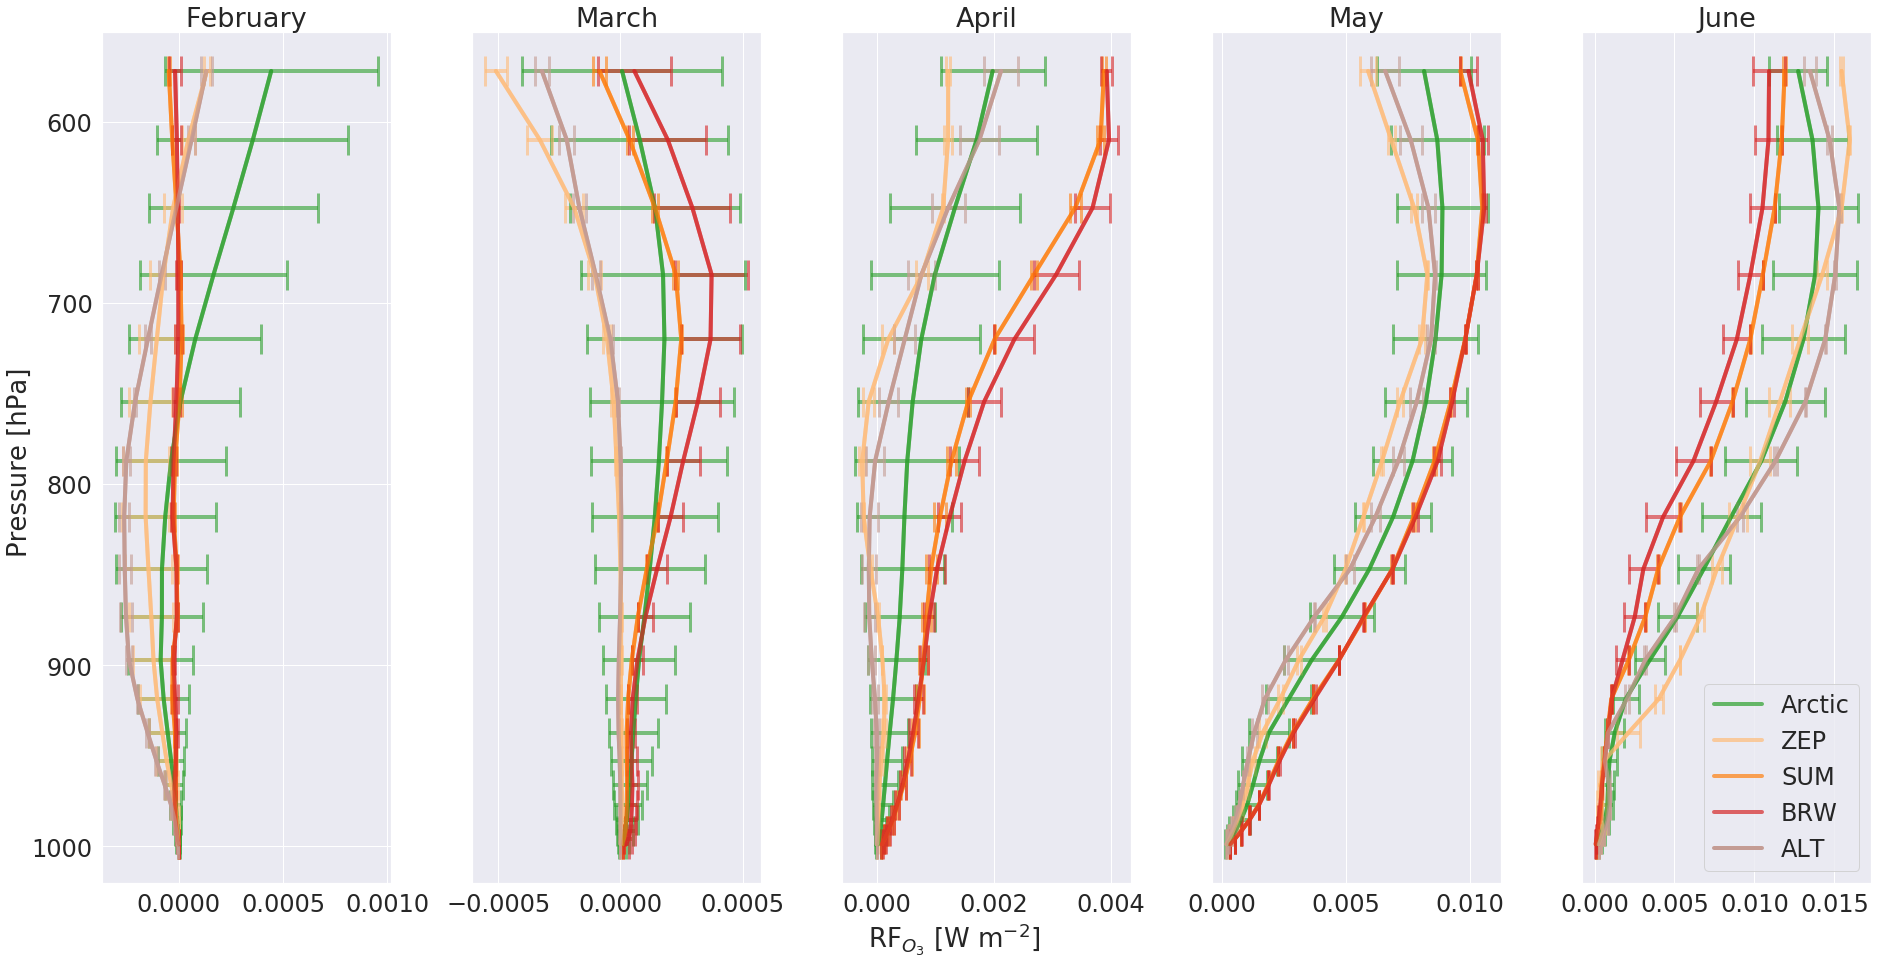
\includegraphics[width = \linewidth]{Chapter6_Results/images/RF/RF_USE/vert_RF_2001_BE.png}
    \caption{Monthly mean averaged RF (in Wm$^{-2}$) using the BE-branch in each model layer (layer 1-60) averaged over the whole Arctic (defined as above 68$^o$N) (green line), over Zeppelin (77.0-80.5$^o$N, 10.5-13.5$^o$E) (yellow line), over Summit (71.0-74.0$^o$N, 40.0-37.0$^o$W)(orange line), over Barrow (70.0-73.0$^o$N, 40.0-37.0$^o$W)(red line) and over Alert (80.5-84.5$^o$N, 64.0-61.0$^o$W)(purple line). Errorbars indicate the standard deviation in the layer. The profiles are shown for the months February-June in 2001}
    \label{fig:vert_RF_2001}
\end{figure}